\documentclass[10pt,a4paper]{article}
\usepackage[top=17mm,bottom=18mm,left=19mm,right=19mm]{geometry}
\usepackage[T1]{fontenc}\usepackage[utf8]{inputenc}
\usepackage{lmodern,microtype,graphicx,booktabs,xcolor,hyperref,amsmath}
\definecolor{ink}{HTML}{193F50}
\hypersetup{colorlinks=true,urlcolor=ink,linkcolor=ink,citecolor=ink,pdftitle={Decoding self-reported distress during emotional videos},pdfauthor={Mathias Chebbah, Aurélien Saint-Grégoire, Ashley Russo}}
\setlength{\parindent}{0pt}\setlength{\parskip}{4pt}
% Derived from results/study11 by scripts/study11_tables.py.
\newcommand{\RidgeGap}{-0.0072\;[-0.0138;\,-0.0003]}
\newcommand{\RidgeGapShort}{-0.007}
\newcommand{\ReveGap}{0.0258\;[0.0137;\,0.0382]}
\newcommand{\RidgeSame}{-0.0129\;[-0.0214;\,-0.0047]}
\newcommand{\ReveSame}{0.0004\;[-0.0088;\,0.0104]}
\newcommand{\RidgeFullGap}{-0.0153\;[-0.0226;\,-0.0087]}
\newcommand{\FourPhase}{0.5694}
\newcommand{\ThreePhase}{0.5655}
\newcommand{\PostDiff}{0.0039\;[-0.0042;\,0.0129]}
\newcommand{\TreeRaw}{0.462}
\newcommand{\TreeSame}{0.505\;[0.491;\,0.519]}
\newcommand{\FoldPrior}{0.427}
\newcommand{\LadderTable}{\begin{tabular}{lccccc}
\toprule
Model & R1 & R2 & R3 & R4 & $\Delta$ R4$-$R1 (95\% CI) \\
\midrule
Multimodal Ridge & $0.577$ & $0.570$ & $0.579$ & $0.569$ & $-0.007\;[-0.014;\,-0.000]$ \\
REVE + Ridge & $0.558$ & $0.557$ & $0.561$ & $0.560$ & $0.002\;[-0.007;\,0.011]$ \\
REVE + logit & $0.538$ & $0.543$ & $0.558$ & $0.564$ & $0.026\;[0.014;\,0.038]$ \\
\bottomrule
\end{tabular}}
\newcommand{\OrderTable}{\begin{tabular}{lccc}
\toprule
Input & AUC (95\% CI) & C1--2 & C3--5 \\
\midrule
Trial index & $0.501\;[0.482;\,0.520]$ & $0.494$ & $0.518$ \\
Cohort $\times$ index & $0.488\;[0.469;\,0.507]$ & $0.484$ & $0.497$ \\
Nominal pre-stimulus & $0.504\;[0.488;\,0.520]$ & $0.504$ & $0.503$ \\
Previous trial & $0.496\;[0.483;\,0.509]$ & $0.492$ & $0.508$ \\
Current clip, no post & $0.566\;[0.551;\,0.579]$ & $0.559$ & $0.582$ \\
\bottomrule
\end{tabular}}
\newcommand{\CalIDs}{21}
\newcommand{\NonRawRows}{41}
\newcommand{\NonRawRecords}{1}
\newcommand{\BeforeQC}{11\,368}
\newcommand{\AfterQC}{11\,002}
\newcommand{\RawIDs}{205}
\newcommand{\RawEvaluable}{203}
\newcommand{\RawRows}{10\,031}
\newcommand{\BodyRMSE}{6.27}
\newcommand{\BodyR}{0.677}
\newcommand{\OrigRMSE}{5.442}
\newcommand{\TreeRMSE}{5.308}
\newcommand{\TreeWithEEG}{5.294}
\newcommand{\TreeGain}{0.0139\;[-0.0084;\,0.0370]}
\newcommand{\TreeGainR}{0.0020\;[-0.0013;\,0.0054]}
\newcommand{\RawOriginalGain}{0.0828\;[0.0490;\,0.1179]}
\newcommand{\ArchiveOriginalGain}{0.0850\;[0.0517;\,0.1190]}
\newcommand{\RawGainR}{0.0006\;[-0.0069;\,0.0083]}
\newcommand{\RawGainRMSE}{0.1085\;[0.0476;\,0.1971]}
\newcommand{\RawGainShort}{0.108}
\newcommand{\RawBefore}{0.037\;[-0.050;\,0.097]}
\newcommand{\RawCleanup}{0.072\;[-0.010;\,0.221]}
\newcommand{\RawVsRelease}{0.067\;[-0.007;\,0.195]}
\newcommand{\ResidualGain}{0.074\;[0.037;\,0.110]}
\newcommand{\StrongBodyImprove}{-0.824\;[-1.829;\,-0.271]}
\newcommand{\ReleaseMatched}{-0.030\;[-0.238;\,0.092]}
\newcommand{\RawOther}{0.051\;[0.040;\,0.061]}
\newcommand{\RawShuffle}{0.047\;[0.037;\,0.058]}
\newcommand{\RawInteraction}{-1.86\;[-3.84;\,-0.14]}
\newcommand{\InteractionN}{182}
\newcommand{\CouplingBefore}{0.128}
\newcommand{\CouplingAfter}{0.131}
\newcommand{\StrictPre}{0.519\;[0.504;\,0.536]}
\newcommand{\StrictPreN}{188}
\newcommand{\BodyTable}{\begin{tabular}{lcc}
\toprule
Model & $r$ & RMSE (bpm) \\
\midrule
Recent RR sequence & $0.517$ & $6.649$ \\
Archived body (57 features) & $0.690$ & $5.442$ \\
Body plus raw trajectories & $0.677$ & $6.266$ \\
Body + bands after ECG regression & $0.677$ & $6.221$ \\
Body + raw REVE & $0.676$ & $6.229$ \\
Body + raw REVE after ECG regression & $0.678$ & $6.157$ \\
Body only, trees & $0.701$ & $5.308$ \\
Body + REVE after ECG regression, trees & $0.703$ & $5.294$ \\
\bottomrule
\end{tabular}}

\title{\vspace{-2em}\Large\bfseries\color{ink} Decoding self-reported distress during emotional videos\\[2pt]\large Matched training budgets and a raw EEG test of cardiac forecasting}
\author{\normalsize Mathias Chebbah \quad Aurélien Saint-Grégoire \quad Ashley Russo\\\small Team 12, Université Paris-Saclay $\times$ HABS Neuro-AI Hackathon\\\small Mentor: Andrew Jeyathasan}
\date{}\begin{document}\maketitle\vspace{-1.5em}
\begin{abstract}\noindent
Across 22,974 emotional-video trials from 314 HABS participant IDs, we tested whether biosignals rank self-reported distress when both IDs and video themes are new. At equal training size, holding out both reduced the multimodal Ridge AUC by 0.0072 (95\% CI for R4 minus R1: $-0.0138$ to $-0.0003$). Trial index alone ranked distress near chance; a strictly pre-onset EEG--body model reached AUC 0.519. In a separate task, adding raw EEG after ECG regression reduced heart-rate-change RMSE by 0.1085 bpm against an enriched but weaker-performing linear body model. Against the best body-only comparator, boosted trees, the paired reduction was $\TreeGain$ bpm. The ECG projection did not reduce the measured scalp coupling. Small predictive gains depend on the comparator, and their cortical origin remains unresolved.
\end{abstract}
\section{Population and outcome}
HABS recorded EEG, ECG, skin conductance, respiration and ratings after written informed consent \cite{habs}. Aligned data cover 314 of 317 labeled IDs (508 recordings, 252 ten-second clips, 84 themes, five cohorts). A person could receive multiple IDs across cohorts. We used development data after an earlier internal holdout was inspected; the 29 organizer-reserved IDs were unavailable.

Distress required valence $\le4$ and arousal $\ge6$ on nine-point scales (5,510 trials, 24.0\%). Videos were randomized in cohorts 1--2 and presented in randomized emotion blocks in cohorts 3--5. Block designs can confound EEG classification with time \cite{li}. We therefore tested session position and previous-trial physiology. An organizer timing advisory led us to exclude the eye streams.
\section{Physiological responses}
The audited development split contained 12,693 trials from 228 IDs and 66 themes. We recomputed the physiological curves on this split. For each one-second bin, we subtracted the trial's three-second prestimulus mean and computed a pooled-SD contrast using at least three finite values per class, ID and bin. Central delta increased in the first second ($d=0.129$), heart rate was lower at 1--2 s ($d=-0.05$), respiratory amplitude was lower at 2--3 s ($d=-0.088$), and conductance was higher at 9--10 s ($d=0.169$). These descriptive profiles do not identify the ordering of physiological onsets. For conductance, all three prestimulus intervals include zero on this split.
\begin{center}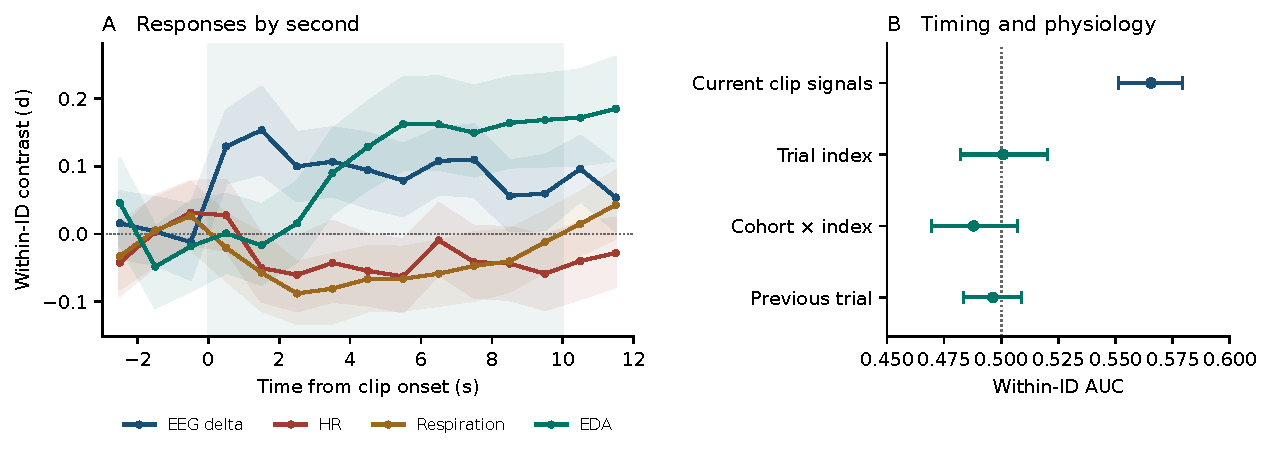
\includegraphics[width=.94\textwidth]{figures/study11_time.pdf}\end{center}
{\small\textbf{Figure 1.} A. Mean contrasts and pointwise 95\% intervals; shaded clip. Per bin, 208 IDs contribute EEG, HR and respiration, and 179--180 contribute EDA (historical split: 235 eligible, 206--208 finite EDA effects under the earlier rule). B. Held-out AUC for current signals, time and prior-trial signals; the last control excludes each session's first aligned trial.}
\clearpage
\section{Generalization at equal training volume}
We ranked distress versus other trials within each ID and averaged the resulting ROC-AUCs over IDs with at least three trials per class ($n=208$). Imputation, scaling, PCA and model selection used training folds. The Ridge head predicts valence and arousal and combines their standardized predictions. Frozen REVE \cite{reve} was evaluated with this head and with logistic regression. Its nominal input is [0,10) s. The 448 engineered features span reference, early, late and post-clip phases, from $-3$ to $+12$ s. The post-clip phase can overlap the rating prompt.

Every regime scored the same nine ID-by-theme test cells. Training pools permitted overlap on both axes (R1), excluded test themes (R2), excluded test IDs (R3), or excluded both (R4). Even R1 excludes the joint test cell: overlap is allowed on each axis separately. Within each cell, all regimes trained on exactly the number of rows available to R4 (mean 5,641 across cells). R1--R3 used ten fixed subsampling seeds shared by models. We averaged each ID's AUC over seeds before calculating paired ID-bootstrap intervals. The full-pool comparison used the same test cells; its R1 is the complement of a cell (about 89\% of development), distinct from the historical 80\% random split.
\begin{center}\small\LadderTable\end{center}
\begin{center}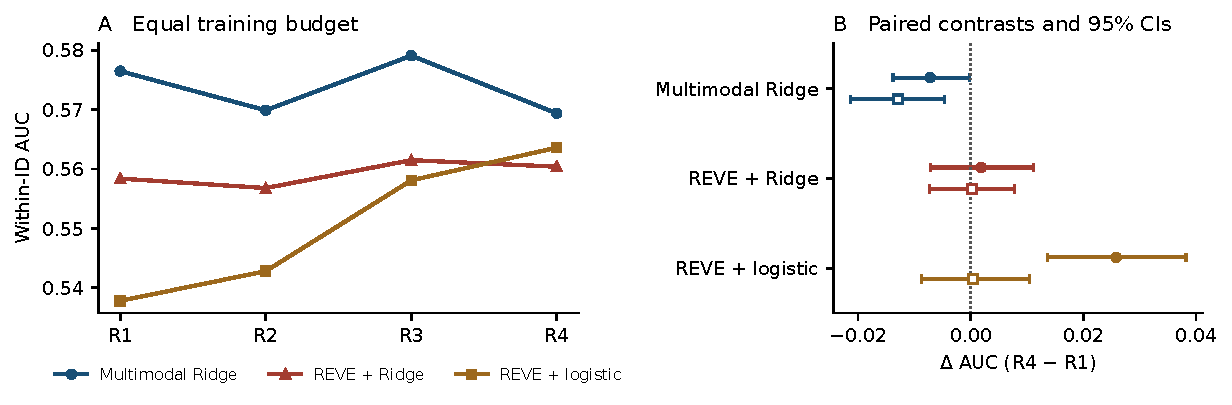
\includegraphics[width=.93\textwidth]{figures/study11_ladder.pdf}\end{center}
{\small\textbf{Figure 2.} Mean within-ID AUC across the four equal-budget regimes (left) and paired R4 minus R1 contrasts with 95\% intervals (right). Filled circles use all within-ID pairs; open squares use only pairs from the same fitted model.}\par
With the full training pools, the paired Ridge contrast was $\RidgeFullGap$. Removing the extra R1 training rows alone cost 0.0082 AUC [0.0047; 0.0116]. The seed-to-seed SD of the matched contrast was 0.0040. A smaller gap remained at equal volume ($\RidgeGap$). The REVE logistic head moved in the opposite direction ($\ReveGap$). A secondary analysis, motivated by the fold-offset control below, compared only trial pairs scored by the same fitted model. The corresponding contrasts were $\RidgeSame$ for multimodal Ridge and $\ReveSame$ for REVE logistic regression. The Ridge drop remains for within-model pairs. The apparent REVE logistic gain largely vanishes. A fixed percentage of the historical decline cannot be attributed to familiar themes across these classifiers.

\textbf{Post-clip ablation.} Removing all 164 features explicitly involving [10,12) s left 284 features. Four-phase Ridge AUC was $\FourPhase$, compared with $\ThreePhase$ without the post phase (paired difference $\PostDiff$). A logistic head benefited more from post-clip features ($+0.0133$ [0.0024; 0.0246]). This ablation tests the contribution of explicit post-clip features. Upstream full-recording filters can still influence earlier values.
\clearpage
\section{Session time and raw cardiac forecasting}
\textbf{Timing controls.} We reconstructed aligned trial order within ID and day before restricting to development themes. The preceding-trial model used unlabeled physiology from the previous aligned trial in the same session. Normalized position assumes session length is known. The table reports the Ridge valence/arousal head; 153 eligible IDs came from cohorts 1--2 and 55 from cohorts 3--5.
\begin{center}\small\OrderTable\end{center}
The nonlinear time classifier's ordinary within-ID AUC was $\TreeRaw$. Some pairs compare predictions across withheld theme folds. A model returning only its training fold's positive rate scored $\FoldPrior$ on these pairs. Restricting comparisons to the same fitted model gave exactly 0.500 for this control and $\TreeSame$ for the nonlinear time classifier. Multimodal inputs extracted from raw prefixes independently cut at stimulus onset yielded $\StrictPre$ ($n=\StrictPreN$). An index-only analysis cannot exclude carryover local to a randomized emotion block.

\textbf{Cardiac target.} We predicted HR in [5,10) s minus HR in [$-3.5$,0) s. The common target uses the archived CURATED ECG extraction. Both beats of each target RR interval fall in [5,10) s; peak detection uses a [4,12) s context on the outcome side. The baseline also has access to that pre-clip reference. This task uses all eligible trials regardless of distress. An enriched body model combines the 57 archived body features, up to 16 recent RR intervals, time since the last beat and half-second summaries of raw ECG, respiration and EDA.

We excluded \NonRawRows{} trials from one recording aligned outside the raw branch. We extracted the 62 EEG channels from \texttt{CURATED}. Original samples were cropped at 5 s before QC, filtered forward (0.5--45 Hz), sampled at 200 Hz and rereferenced across valid electrodes. Trials required at least 50 valid electrodes (peak-to-peak $\le800\,\mu$V, SD $\ge0.01\,\mu$V); all compared models used the same retained rows. REVE received [$-3.2$,5) s. We learned a fixed, channel-specific 0--120 ms ECG lag regression on \CalIDs{} development IDs reserved exclusively for calibration. These IDs never entered predictive CV. Perturbing the samples at and after the cutoff left the tested features and frozen encoder outputs unchanged, with a separate check at 0 s for the pre-onset branch. The comparison between release, raw and ECG-corrected raw representations used identical trials, targets and outer folds.
\begin{center}\small\BodyTable\end{center}
Of \BeforeQC{} evaluation trials before raw QC, \AfterQC{} had usable raw signals. The cardiac comparison retained \RawRows{} common trials from \RawIDs{} IDs; \RawEvaluable{} IDs had sufficient data for the primary within-ID comparison. The primary endpoint was paired RMSE reduction in bpm relative to the enriched body-only Ridge, with positive values indicating smaller errors. Correlation gain measures a change in within-ID linear association.
\clearpage
\section{What adds information about future heart rate?}
\begin{center}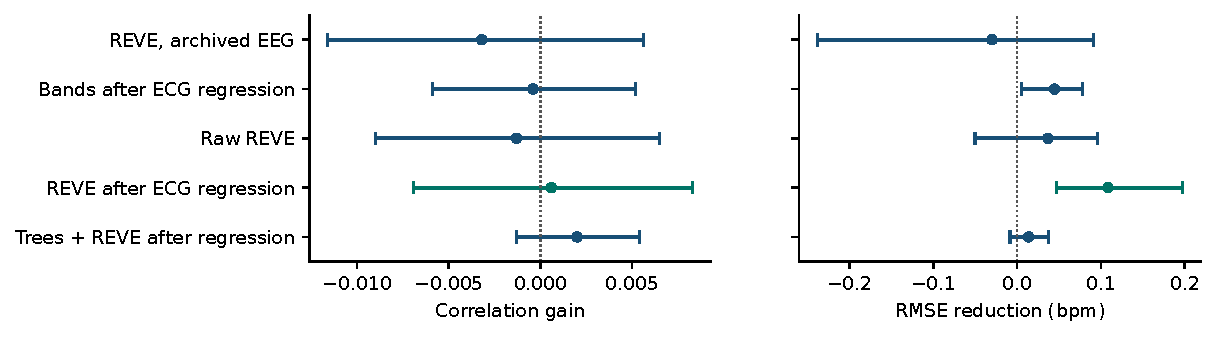
\includegraphics[width=.91\textwidth]{figures/study11_cardiac.pdf}\end{center}
{\small\textbf{Figure 3.} Increment over the corresponding body-only regressor on common trials. The first row uses the archived EEG branch, which preferred the full-recording-preprocessed release and allowed a raw fallback; the other rows require raw EEG. The final row uses boosted trees for both regressors. Intervals resample IDs and condition on the stimulus set.}\par
With the original 57 body features, the held-out RMSE reduction was $\ArchiveOriginalGain$ bpm for archived REVE and $\RawOriginalGain$ for uncorrected raw REVE. Thus the small increment against that reference also occurs on a prefix-limited raw signal. Expanding the body inputs increased linear Ridge RMSE from $\OrigRMSE$ to $\BodyRMSE$ bpm. Against this weaker-performing linear fit, adding raw REVE after ECG regression reduced RMSE by $\RawGainRMSE$ bpm, with correlation gain $\RawGainR$. Allowing a zero EEG weight in a separate residual fit gave an RMSE reduction of $\ResidualGain$ bpm. The best body-only comparator was the boosted-tree model ($\TreeRMSE$ bpm); adding REVE yielded $\TreeWithEEG$ bpm, a paired reduction of $\TreeGain$ bpm. The interval includes no improvement. The evidence for additional EEG information depends on the comparator and outcome metric.

The real-minus-permuted EEG contrast in correlation was $\RawOther$ when the donor was a different ID watching the same clip. For within-ID trial shuffling it was $\RawShuffle$. The difference in squared-error benefit between distress and other trials was $\RawInteraction$ bpm$^2$ ($n=\InteractionN$ IDs). The negative interaction estimate indicates a smaller observed squared-error benefit during distress; the comparison is exploratory. The ECG projection changed the across-ID mean of median absolute zero-lag ECG--EEG correlations from $\CouplingBefore$ to $\CouplingAfter$. Measured coupling did not decrease. The regression cannot establish removal of the cardiac field. Residual artefacts and common physiological drive remain possible. The electrical field of the heart is measurable at scalp electrodes \cite{dirlich}; ECG regression can also attenuate genuinely cardiac-locked neural activity. The enriched body model still summarizes the waveforms; any incremental EEG finding is conditional on that representation.

\textbf{Scope.} These findings concern self-reported affect during laboratory video viewing and a separate forecasting task. Clinical pain, naturally occurring distress and continuous alarms require different validation. Matching the number of training examples does not fix class balance, theme composition or the number of distinct IDs across regimes. The supplement documents the earlier same-video comparisons, fear and disgust, cardiac-evoked potentials, Varimax PCA, CORAL and known-class averaging.
\textbf{Data and code.} Individual recordings are available by application to HABS. Aggregate estimates, code, source revisions and run identifiers are in the \href{https://github.com/mathiaschebbah/habs}{team repository}.
\begin{thebibliography}{4}\small
\bibitem{habs} HABS NeuroAI team. \emph{A large EEG dataset with ECG, skin conductance, respiration, gaze and pupillometry for emotion decoding}. 2026. \href{https://huggingface.co/datasets/HABSteam/multimodal-eeg-emotion}{Dataset}.
\bibitem{reve} Y. El Ouahidi et al. REVE: A Foundation Model for EEG --- Adapting to Any Setup with Large-Scale Pretraining on 25,000 Subjects. \emph{NeurIPS}, 2025. \href{https://arxiv.org/abs/2510.21585}{arXiv:2510.21585}.
\bibitem{li} R. Li et al. The Perils and Pitfalls of Block Design for EEG Classification Experiments. \emph{IEEE TPAMI}. \href{https://doi.org/10.1109/TPAMI.2020.2973153}{doi:10.1109/TPAMI.2020.2973153}.
\bibitem{dirlich} G. Dirlich, L. Vogl, M. Plaschke, F. Strian. Cardiac field effects on the EEG. \emph{Electroencephalogr. Clin. Neurophysiol.} 102, 307--315 (1997). \href{https://pubmed.ncbi.nlm.nih.gov/9146492/}{PMID 9146492}.
\end{thebibliography}\end{document}
